% arara: xelatex
%% arara: xelatex


% https://koalatea.io/r-knn-regression/
% http://freerangestats.info/blog/2017/04/09/propensity-v-regression
% https://economics.stackexchange.com/questions/45335/what-is-the-difference-between-ate-and-att
% https://kosukeimai.github.io/MatchIt/articles/matching-methods.html


\documentclass[14pt,xcolor=dvipsnames]{beamer}


% !TEX root = om_metrics_14.tex

%\usepackage{epsdice} % dice 1-6 for probability :)

% \usepackage[absolute,overlay]{textpos}

% \usefonttheme[onlymath]{serif}

\usefonttheme{professionalfonts}
% by default beamer changes math fonts for better visibility for projection
% this professionalfonst theme removes this behavior


\usepackage[orientation=portrait,size=custom,width=25.4,height=19.05]{beamerposter}




%25,4 см 19,05 см размеры слайда в powerpoint

\usetheme{metropolis}
\metroset{
  %progressbar=none,
  numbering=none,
  subsectionpage=progressbar,
  block=fill
}

%\usecolortheme{seahorse}

\usepackage{fontspec}
\usepackage{polyglossia}
\setmainlanguage{english}


% \usepackage{fontawesome5} % removed [fixed]
\setmainfont[Ligatures=TeX]{Myriad Pro}
% \setsansfont{Myriad Pro}




% why do we need \newfontfamily:
% http://tex.stackexchange.com/questions/91507/
\newfontfamily{\cyrillicfonttt}{Myriad Pro}
\newfontfamily{\cyrillicfont}{Myriad Pro}
%\newfontfamily{\cyrillicfontbs}{Myriad Pro}
\newfontfamily{\cyrillicfontsf}{Myriad Pro}


% https://tex.stackexchange.com/questions/175860/why-does-unicode-math-break-the-kerning-of-accents-in-combination-with-amssymb
% "You shouldn't be using amssymb together with unicode-math"
\usepackage{amsmath}
\usepackage{amsthm} % amssymb 


% https://tex.stackexchange.com/questions/483722/
% \usepackage[MnSymbol]{mathspec}  % Includes amsmath.
% \usepackage{mathspec}  % Includes amsmath.
% \setmathsfont(Digits,Latin,Greek,Symbols)[Numbers={Lining,Proportional}]{Latin Modern Math}
% mathspec must be loaded earlier than amsmath



%\usepackage{bm}

% \usepackage{fdsymbol} % \nperp

% \usepackage{unicode-math} % \symbf
% \setmathfont{Latin Modern Math}



\usepackage{centernot}

\usepackage{graphicx}

\usepackage{wrapfig}
% \usepackage{animate} % animations :)
% \usepackage{tikz}
%\usetikzlibrary{shapes.geometric,patterns,positioning,matrix,calc,arrows,shapes,fit,decorations,decorations.pathmorphing}
% \usepackage{pifont}
\usepackage{comment}
\usepackage[font=small,labelfont=bf]{caption}
\captionsetup[figure]{labelformat=empty}
% \includecomment{techno}



%Расположение

\setbeamersize{text margin left=15 mm,text margin right=5mm} 
\setlength{\leftmargini}{38 pt}

%\usepackage{showframe}
%\usepackage{enumitem}
% \setlist{leftmargin=5.5mm}


%Цвета от дирекции

\definecolor{dirblack}{RGB}{58, 58, 58}
\definecolor{dirwhite}{RGB}{245, 245, 245}
\definecolor{dirred}{RGB}{149, 55, 53}
\definecolor{dirblue}{RGB}{0, 90, 171}
\definecolor{dirorange}{RGB}{235, 143, 76}
\definecolor{dirlightblue}{RGB}{75, 172, 198}
\definecolor{dirgreen}{RGB}{155, 187, 89}
\definecolor{dircomment}{RGB}{128, 100, 162}

\setbeamercolor{title separator}{bg=dirlightblue!50, fg=dirblue}

%Цвета блоков

% Голубой блок!
\setbeamercolor{block title}{bg=dirblue!30,fg=dirblack}
\setbeamercolor{block title example}{bg=dirlightblue!50,fg=dirblack}
\setbeamercolor{block body example}{bg=dirlightblue!20,fg=dirblack}

\AtBeginEnvironment{exampleblock}{\setbeamercolor{itemize item}{fg=dirblack}}
%\setbeamertemplate{blocks}[rounded][shadow]

% Набор команд для удобства верстки

% Набор команд для структуризации

%\newcommand{\quest}{\faQuestionCircleO}
%\faPencilSquareO \faPuzzlePiece \faQuestionCircleO  \faIcon*[regular]{file} {\textcolor{dirblue}
%\newcommand{\quest}{\textcolor{dirblue}{\boxed{\textbf{?}}}
%\newcommand{\task}{\faIcon{tasks}}
%\newcommand{\exmpl}{\faPuzzlePiece}
%\newcommand{\dfn}{\faIcon{pen-square}}
%\newcommand{\quest}{\textcolor{dirblue}{\faQuestionCircle[regular]}}
%\newcommand{\acc}[1]{\textcolor{dirred}{#1}}
%\newcommand{\accm}[1]{\textcolor{dirred}{#1}}
%\newcommand{\acct}[1]{\textcolor{dirblue}{#1}}
%\newcommand{\acctm}[1]{\textcolor{dirblue}{#1}}
%\newcommand{\accex}[1]{\textcolor{dirblack}{\bf #1}}
%\newcommand{\accexm}[1]{\textcolor{dirblack}{ \mathbf{#1}}}
%\newcommand{\acclp}[1]{\textcolor{dirorange}{\it #1}}
\newcommand{\todo}[1]{\textcolor{dircomment}{\bf #1}}
%\newcommand{\graylink}[1]{{\fontsize{11}{12}\selectfont \textcolor{gray}{#1}}}
%\newcommand{\figcaption}[1]{{\fontsize{18}{20}\selectfont #1}}


\newcommand{\videotitle}[1]{
    {\fontsize{33}{30}\selectfont \textcolor{dirblue}{\textbf{#1}} }

    %\todo{название видеофрагмента}
}

\newcommand{\lecturetitle}[1]{
  {\fontsize{33}{30}\selectfont \textcolor{dirblue}{\textbf{#1}} }

    %\todo{название лекции}
}





%\newcommand{\spcbig}{\vspace{-10 pt}}
%\newcommand{\spcsmall}{\vspace{-5 pt}}

%\usepackage{listings}
%\lstset{
%xleftmargin=0 pt,
%  basicstyle=\small, 
%  language=Python,
  %tabsize = 2,
%  backgroundcolor=\color{mc!20!white}
%}



%\newcommand{\mypart}[1]{\begin{frame}[standout]{\huge #1}\end{frame}}

\setbeamercolor{background canvas}{bg=}

% frame title setup
\setbeamercolor{frametitle}{bg=,fg=dirblue}
\setbeamertemplate{frametitle}[default][left]

\addtobeamertemplate{frametitle}{\hspace*{0.1 cm}}{\vspace*{0.25cm}}


%Шрифты
\setbeamerfont{frametitle}{family=\rmfamily,series=\bfseries,size={\fontsize{33}{30}}}
\setbeamerfont{framesubtitle}{family=\rmfamily,series=\bfseries,size={\fontsize{26}{20}}}


% удобнее знать номер слайда, чтобы вносить правки!  

\setbeamercolor{footline}{fg=dircomment}
\setbeamerfont{footline}{series=\bfseries, size={\fontsize{12}{14}}}
%\setbeamertemplate{footline}[page number]


\defbeamertemplate{footline}{custom footline}
{%
  \hspace*{\fill}%
  \usebeamercolor[fg]{page number in head/foot}%
  \usebeamerfont{page number in head/foot}%
  page: \insertpagenumber\,/\,\insertpresentationendpage%
  \hspace{20pt}%
  slide: \insertframenumber\,/\,\inserttotalframenumber%
  %\hspace*{\fill}
  \vskip2pt%
}
%\setbeamertemplate{footline}[custom footline]

\usepackage{physics}



% tikz block

\usepackage{pgfplots}
\pgfplotsset{compat=newest}

\usepackage{tikz}
\usetikzlibrary{calc}
\usetikzlibrary{quotes,angles}
\usetikzlibrary{arrows}
\usetikzlibrary{arrows.meta}
\usetikzlibrary{positioning,intersections,decorations.markings}
\usetikzlibrary{patterns}
\usepackage{tikzsymbols}

\usepackage{tkz-euclide} 
%\tikzset{>=latex}

\tikzset{cross/.style={cross out, draw=black, minimum size=2*(#1-\pgflinewidth), inner sep=0pt, outer sep=0pt},
%default radius will be 1pt. 
cross/.default={5pt}}

\colorlet{veca}{red}
\colorlet{vecb}{blue}
\colorlet{vecc}{olive}


\newcommand{\grid}{\draw[color=gray,step=1.0,dotted] (-2.1,-2.1) grid (9.6,6.1)}

% end tikz block

\newcommand{\R}{\mathbb{R}}
\newcommand{\Rot}{\mathrm{R}}
\newcommand{\HH}{\mathrm{H}}
\newcommand{\Id}{\mathrm{I}}
\newcommand{\RR}{\mathbb{R}}
\newcommand{\ZZ}{\mathbb{Z}}
\newcommand{\la}{\lambda}
\let\P\relax
\newcommand{\P}{\mathbb{P}}
\newcommand{\E}{\mathbb{E}}

\newcommand{\cN}{\mathcal{N}}
\newcommand{\dN}{\mathcal{N}}

\newcommand{\qL}{q_{\text{left}}}
\newcommand{\qR}{q_{\text{right}}}



\newcommand{\ba}{\mathbf{a}}
\newcommand{\be}{\mathbf{e}}
\newcommand{\bb}{\mathbf{b}}
\newcommand{\bc}{\mathbf{c}}
\newcommand{\bd}{\mathbf{d}}
\newcommand{\bx}{\mathbf{x}}
\newcommand{\bff}{\mathbf{f}} % \bf is already def
\newcommand{\bv}{\mathbf{v}}
\newcommand{\bzero}{\mathbf{0}}


\DeclareMathOperator{\Var}{Var}
\DeclareMathOperator{\sVar}{sVar}
\DeclareMathOperator{\Cov}{Cov}
\DeclareMathOperator{\sCov}{sCov}
\DeclareMathOperator{\sCorr}{sCorr}
\DeclareMathOperator{\Corr}{Corr}

\DeclareMathOperator{\plim}{plim}


\newcommand{\graylink}[1]{{\fontsize{11}{12}\selectfont \textcolor{gray}{#1}}}
\newcommand{\figcaption}[1]{{\fontsize{18}{20}\selectfont #1}}





\begin{document}


\begin{frame} % название лекции


\lecturetitle{Wiener process and martingales}

\end{frame}


% !TEX root = ../coursera_sc_01.tex

\begin{frame} % название фрагмента

\videotitle{Wiener process}

\end{frame}


\begin{frame}{Stochastic calculus course}
  The goal: price an option in the framework of Black and Scholes model. 

  \begin{itemize}[<+->]
    \item Very short: \alert{4 weeks} only.
    \item Mathematics is \alert{hard}.
    \item \alert{Informal} definitions and theorems. 
    \item \alert{Problem solving} and computer \alert{simulations}. 
  \end{itemize}

\end{frame}


\begin{frame}{Wiener process}

  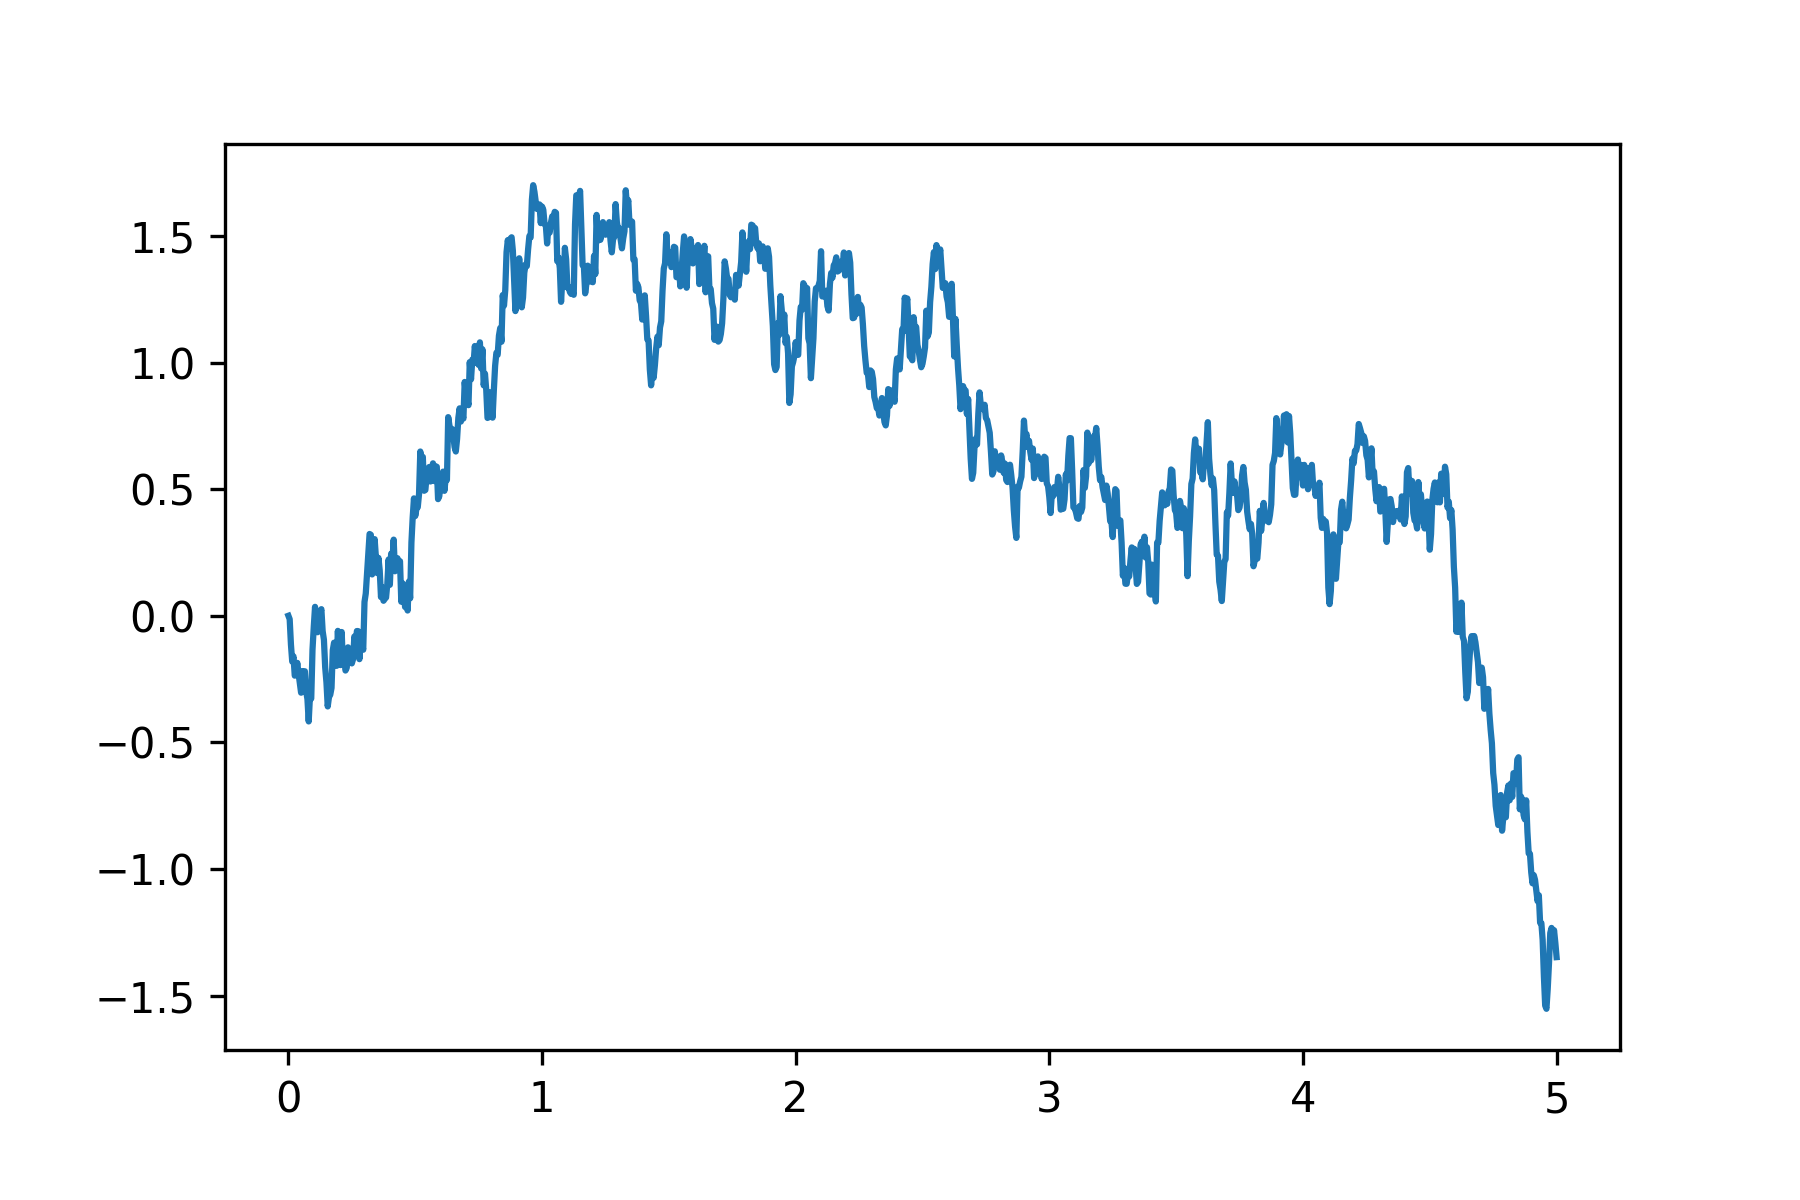
\includegraphics[width=\textwidth]{pictures/wiener_process.png}


\end{frame}


\begin{frame}{Stochastic process}

  \begin{block}{Definition \formalduck}
    \alert{Stochastic} or \alert{random process} is a collection of random variables indexed by time variable $t$. 
    \pause

    \alert{Continuous time}: $(X_t, t\geq 0)$.
    \pause 
    
    \alert{Discrete time}: $(X_t, t\in \{0, 1, 2, 3, \ldots \})$. 
\end{block}

\pause 
Notation remark:
\begin{itemize}[<+->]
  \item $(X_t, t\geq 0)$ or $(X_t)$ — collection of random variables;
  \item $X_t$ — one particular random variable. 
\end{itemize}


\end{frame}

\begin{frame}
  \frametitle{Wiener process}

  \begin{block}{Definition\formalduck}
    Stochastic process $(W_t, t\geq 0)$ is called \alert{Wiener process} or \alert{Brownian motion} if 
    \pause
    \begin{enumerate}[<+->]
      \item $W_0 = 0$.
      \item Increments $W_t - W_s$ are normally distributed $\cN(0; t-s)$. 
      \item Increment $W_t - W_s$ is independent of the past values $(W_u, u\leq s)$.
      \item $\P(\text{trajectory of } (W_t) \text{ is continuous} ) = 1$.
  \end{enumerate}
  
  \end{block}

  \pause 
  Tradition: when we consider two arbitrary moments of time, $s$ and $t$, we usually assume $s \leq t$. 
\end{frame}

\begin{frame}
  \frametitle{Divide and conquer}

  The main trick to study properties:
  \[
  \text{\alert{Future value}} = \text{\alert{Known value}} + \text{\alert{Unpredictable change}}  
  \]
  \pause 
  Seems trivial\harlequinduck
  \[
  W_t = W_s + (W_t - W_s)  
  \]

\end{frame}


\begin{frame}
\frametitle{Conditional probability exercise}
Exercise\knightduck. Calculate $\P(W_{10} > 2 \mid W_6 = 3)$.
\begin{align*}
  \onslide<2->{&\P(W_{10} > 2 \mid W_6 = 3) = \P(W_{10} - W_6 + W_6 >2 \mid W_6 = 3) = } \\
  \onslide<3->{&= \P(W_{10} - W_6 + 3 >2 \mid W_6 = 3) = \P(W_{10} - W_6 > -1)}.
\end{align*}
\[
\onslide<4->{W_{10} - W_6 \sim \cN(0;4), \pause \text{ hence } \frac{W_{10} - W_6 - 0 }{\sqrt{4}} \sim \cN(0;1)}. 
\]

\onslide<5->{We will use standard normal distribution function $F(u) = \P(Z \leq u)$, where $Z\sim \cN(0;1)$.}
\begin{align*}
  \onslide<6->{\P(W_{10} - W_6 > -1) = \P\left(\frac{W_{10} - W_6}{2} > -\frac{1}{2}\right)  = }\\
  \onslide<7>{= \P(Z > -0.5) = \P(Z < 0.5) = F(0.5) \pause \approx 0.69.}
\end{align*}


\end{frame}


\begin{frame}
  \frametitle{More gentlemen's agreements}

  On slides we will follow these agreements:
  \begin{itemize}[<+->]
    \item $s$ and $t$ denote two arbitrary time moments with $0 \leq s \leq t$.
    \item $(W_t)$ denotes a Wiener process.
    \item $Z$ denotes a standard normal random variable, $Z \sim \cN(0;1)$.
    \item $F(u)$ denotes the standard normal distribution function, $F(u) = \P(Z \leq u)$.
  \end{itemize}
  

\end{frame}



\begin{frame}
  \frametitle{Independence of increments: example}
  \begin{block}{Property}
    Increment $W_t - W_s$ is independent of the past values $(W_u, u\leq s)$.  
  \end{block}

  \pause 
  $W_6 - W_4$ is independend of $W_4$, $W_{3}$, $W_{2.5}$, $W_1$, \ldots 

  \pause 
  $W_6 - W_4$ is independent of $W_4 - W_3$, $W_{2.5} - W_{1}$.

  \pause
  The increments $W_6 - W_4$, $W_4 - W_3$, $W_{2.5} - W_1$ are independent. 

\end{frame}


\begin{frame}
  \frametitle{Independence of increments: full glory}


  If the time intervals $[s_1, t_1]$, $[s_2, t_2]$, \ldots, $[s_k, t_k]$ are
  \alert{non overlapping},

  \begin{center}
    \begin{tikzpicture}
      \coordinate (a) at (-3,0);
      \coordinate (b) at (14,0);

      \coordinate [label=below:$s_1$] (s1) at (0,0);
      \coordinate [label=below:$t_1$] (t1) at (2,0);
      \coordinate [label=below:$s_2$] (s2) at (3,0);
      \coordinate [label=below:$t_2$] (t2) at (6,0);
      \coordinate [label=below:$s_k$] (sn) at (10,0);
      \coordinate [label=below:$t_k$] (tn) at (12,0);  



      \draw[line width=1pt, black, -stealth] (a)--(8,0);
      \draw[line width=1pt, black, stealth reversed-] (8.5,0)--(b);

      \filldraw [blue] (s1) circle[radius=3pt];
      \filldraw [blue] (t1) circle[radius=3pt];
      \filldraw [blue] (s2) circle[radius=3pt];
      \filldraw [blue] (t2) circle[radius=3pt];
      \filldraw [blue] (sn) circle[radius=3pt];
      \filldraw [blue] (tn) circle[radius=3pt];

      \draw[line width=4pt, blue] (s1)--(t1);
      \draw[line width=4pt, blue] (s2)--(t2);
      \draw[line width=4pt, blue] (sn)--(tn);     
    \end{tikzpicture}
  \end{center}
  

  \pause 
  then the increments $W(t_1) - W(s_1)$, $W(t_2) - W(s_2)$, \ldots, $W(t_k) - W(s_k)$ are independent. 

  \pause
  Remark: the right border of an interval \alert{may touch} the left border of the next one,
  but \alert{may not exceed} it, $t_j \leq s_{j+1}$. 

\end{frame}


\begin{frame}
  \frametitle{Expectation and variance}

  Exercise\knightduck. Find $\E(W_t)$, $\Var(W_t)$, $\Cov(W_s, W_t)$.
  \begin{flalign*}
    \onslide<2->{\E(W_t) &= \E(W_t - W_0) = 0&}    
  \end{flalign*}
  \begin{flalign*}
  \onslide<3->{\Var(W_t) &= \Var(W_t - W_0) = t - 0 = t&}
\end{flalign*}  
  \onslide<4->{For $t\geq s$:}
  \begin{flalign*}  
  \onslide<5->{\Cov(W_s, W_t) &= \Cov(W_s, W_s + (W_t - W_s)) = \Cov(W_s,W_s) = s&}
\end{flalign*}
\begin{flalign*}
    \onslide<6>{\Cov(W_7, W_3) &= 3.&}  
  \end{flalign*}

\end{frame}


\begin{frame}{Two friends}

  \begin{block}{Definition\formalduck}
    Stochastic process $(X_t, t\geq 0)$ that may be written as
    \[
    X_t = a W_t + b t,  
    \]
    is called \alert{brownian motion with drift and scaling}.
  \end{block}

  \pause
  \begin{block}{Definition\formalduck}
    Stochastic process $(S_t, t\geq 0)$ that may be written as
    \[
    S_t = S_0 \exp(a W_t + b t),
    \]
    is called \alert{geometric brownian motion}.
  \end{block}
  
\end{frame}


\begin{frame}{Two plots}

  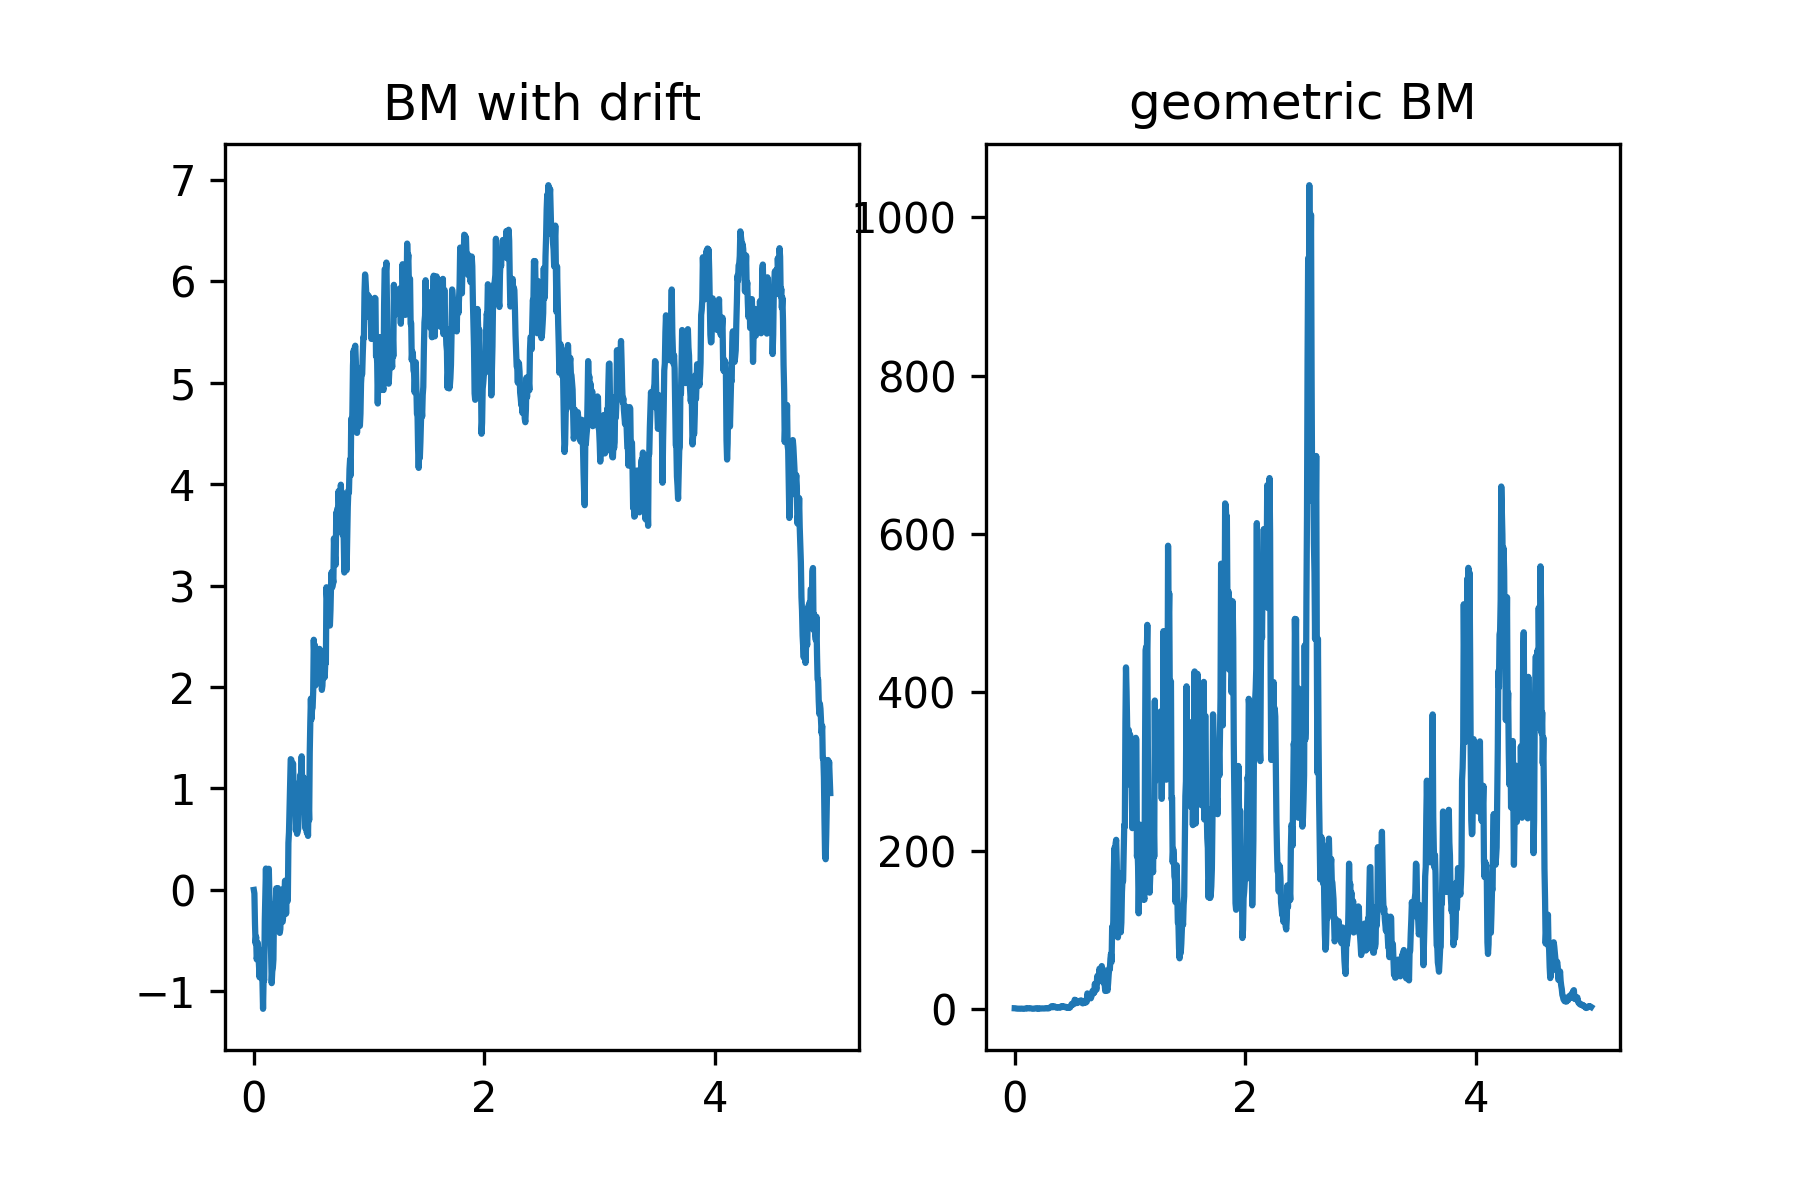
\includegraphics[width=\textwidth]{pictures/two_wiener_friends.png}

\end{frame}


\begin{frame}
  \frametitle{BM with drift and scaling}

  Exercise\knightduck. Find $\E(5W_t + 6t)$ and $\Var(5W_t + 6t)$.
  
  \begin{flalign*}    
  \onslide<2->{\E(5W_t + 6t) &= 0 + 6t = 6t&}
  \end{flalign*}
  \begin{flalign*}    
    \onslide<3->{\Var(5W_t + 6t) &= \Var(5W_t) = 25t&}
  \end{flalign*}

\end{frame}

\begin{frame}
  \frametitle{Frequently used expected values}

  \onslide<1->{Expected values of exponents:}
  \pause
  \begin{itemize}[<+->]
    \item $\E(\exp(aZ)) = \exp(a^2/2)$ for $Z \sim \cN(0;1)$.
    \item $\E(\exp(aW_t)) = \exp(a^2t/2)$ for Wiener process $W_t$.
  \end{itemize}
  
  \onslide<4->{
  \begin{block}{How these are obtained?\formalduck}
    \pause
    \begin{flalign*}
      \E(\exp(aZ)) &= \int_{-\infty}^{+\infty} \exp(az) f(z) \,dz = &\\
      & = \int_{-\infty}^{+\infty} \exp(az) \frac{1}{\sqrt{2\pi}}\exp(-z^2/2) \,dz&
    \end{flalign*}
  \end{block}
  }

\end{frame}


\begin{frame}
  \frametitle{Moment generating function}

\begin{block}{Definition\formalduck}
  The \alert{moment generating function} (MGF) of a random variable $X$ is defined as 
  \[
  M_X(a) = \E(\exp(a X)).
  \] 
\end{block}

\pause 

\begin{itemize}[<+->]
  \item $M_Z(a) = \exp(a^2/2)$ for a normal $Z \sim \cN(0;1)$.
  \item $M_{W_t}(a)= \exp(a^2t/2)$ for a Wiener process $W_t$.
\end{itemize}
  
\end{frame}

\begin{frame}
    \frametitle{Why may we need MGF?}
    \[
    \onslide<1->{M'(u) = \frac{d}{du}\E(\exp(uX)) =\E(X\exp(uX)) }
    \]
    \[
    \onslide<2->{M'(0) = \E(X)}  
    \]
    \onslide<3->{MGF is a funny\harlequinduck { } way to calculate expected value!}
    \begin{align*}
      \onslide<4->{M''(0) &= \E(X^2)& } \\
      \onslide<5->{M'''(0) &= \E(X^3)&  } \\
      \onslide<6->{&\vdots}      \\
      \onslide<7->{M^{(k)}(0) &= \E(X^k)&}      
    \end{align*}
  
  \end{frame}

\begin{frame}{Wiener process: summary}

\begin{itemize}[<+->]
    \item Stochastic process with \alert{normal} and \alert{independent increments}.
    \item Wiener process with \alert{drift} and \alert{geometric Wiener process}. 
    \item \alert{Moment generating function}. 
\end{itemize}
  
\end{frame}


% !TEX root = ../coursera_sc_01.tex

\begin{frame} % название фрагмента

    \videotitle{Conditional expectation}
    
\end{frame}
    
    
\begin{frame}{Conditional expectation: short plan}
    
      \begin{itemize}[<+->]
        \item Modeling information using \alert{sigma-algebras};
        \item \alert{Properties} of conditional expected value;
        \item Conditional \alert{variance}.
      \end{itemize}
    
\end{frame}
    
    
\begin{frame}{Modeling information}
    
    \onslide<2->{John knows the value of $X$.}

    \onslide<3->{Maria knows the value of $X$ and $Y$.}

    \onslide<4->{Maria knows \alert{more}!}

    \onslide<5->{How to model this \alert{mathematically?}}
    
\end{frame}



\begin{frame}
    \frametitle{Sigma-algebra}

    \pause
    \begin{block}{Definition \informalduck}
        \alert{Sigma-algebra} ($\sigma$-algebra) generated by random variables $X$ and $Y$ is the collection 
        of all events that can be stated in terms of these random variables. 
        
        \pause
        Notation: $\sigma(X, Y)$.
    \end{block}

    \pause
    \begin{block}{Example}
    The sigma-algebra $\sigma(X, Y)$ contains the events $\{X < 5\}$, $\{X > 2Y\}$, $\{\sin Y > \cos X\}$, \ldots
    \end{block}    

\end{frame}


\begin{frame}{Modeling information}
    
    \onslide<2->{John knows the value of $X$, $\cF_J =\sigma (X)$.}

    \onslide<3->{Maria knows the value of $X$ and $Y$, $\cF_M = \sigma (X, Y)$}

    \onslide<4->{Maria knows \alert{more}: $\cF_J \subset \cF_M$.}
    
\end{frame}



\begin{frame}
    \frametitle{Measurability}

    \pause
    \begin{block}{Definition \formalduck}
        The random variable $Z$ is measurable with respect to $\sigma$-algebra $\cF$ if 
        $\sigma(Z) \subset \cF$. 
    \end{block}
    \pause
    Information in $\cF$ is sufficient to calculate the value of $Z$.
    \pause
    \begin{block}{Theorem \informalduck}
        The random variable $Z$ is measurable with respect to $\sigma(X, Y)$ if and only if
        $Z$ is a deterministic function of $X$ and $Y$.  
    \end{block}
\end{frame}


\begin{frame}
    \frametitle{Best prediction}

    \begin{block}{Definition \informalduck}
        The \alert{best prediction} of a random variable $Y$ given $\sigma$-algebra $\cF$ is called 
        \alert{conditional expected value} $\E(Z \mid \cF)$.
    \end{block}

    \pause 
    \begin{block}{Difference of $\E(Z \mid \cF)$ and $\E(Z)$}
    If I know $X$ and $Y$ then my best prediction of $Z$ may depend on $X$ and $Y$.

    In general: $\E(Z \mid \cF)$ is a \alert{random variable}.
    \end{block}
\end{frame}


\begin{frame}
    \frametitle{Notation}

    \begin{itemize}[<+->]
        \item $\alert{\E(Z \mid \cF)}$: 
        
        for a general $\sigma$-algebra $\cF$;
        \item $\E(Z \mid \sigma(X, Y))$ or $\alert{\E(Z \mid X, Y)}$: 
        
        for $\sigma$-algebra generated by $X$ and $Y$.
    \end{itemize}
\end{frame}

\begin{frame}
    \frametitle{When we may omit conditioning?}

    \begin{itemize}[<+->]

        \item If $Z$ is \alert{independend} of $X$ and $Y$ then $\E(Z \mid X, Y) = \E(Z)$:

        If I know \alert{nothing useful} about $Z$ then I can drop my information. 

        \item $\E( \E( Z \mid \cF) ) = \E(Z)$:
        
        The \alert{average of best guess} is the average of predicted variable. 

    \end{itemize}

\end{frame}




\begin{frame}
    \frametitle{The case of known variable}

    If $Z$ is \alert{known} (measurable with respect to $\cF$), 
    then we may treat $Z$ \textit{like} a constant:

    \[
        \onslide<2->{\E(Z \mid \cF ) = Z;}
    \]
    \[
        \onslide<3->{\E(2\exp(5W_t) \mid W_t) = 2\exp(5W_t);}
    \]
    \[
        \onslide<4->{\E(2Z R + Z^2 \mid \cF ) = 2Z \E(R\mid \cF) + Z^2.}
    \]


\end{frame}


\begin{frame}
    \frametitle{Conditional variance}

    \begin{block}{Definition \formalduck}
        The \alert{conditional variance} $\Var(Z \mid \cF)$ is the conditional expected value of the 
        squared error of the best prediction,
        \pause
        \[
            \Var(Z \mid \cF) = \E(\Delta^2 \mid \cF), \text{ where } \Delta = Z - \E(Z \mid \cF).
        \]
    \end{block}

    \pause 
    \begin{block}{Theorem \formalduck}
        \[
            \Var(Z \mid \cF) = \E(Z^2 \mid \cF) - (\E(Z \mid \cF) )^2.
        \]
    \end{block}
\end{frame}




\begin{frame}
    \frametitle{Properties of conditional variance}

    \begin{itemize}[<+->]
        \item Irrelevant information may be omitted:
        
        If $Z$ is \alert{independent} of $\cF$ then $\E(Z \mid \cF) = \E(Z)$ and $\Var(Z \mid \cF) = \Var(Z)$.
        

        \item If $Z$ is \alert{known} (measurable with respect to $\cF$), 
        then we may treat $Z$ \textit{like} a constant:
        \[
            \onslide<3->{\Var(2\exp(5W_t) \mid W_t) = 0;}
        \]
        \[
            \onslide<4->{\Var(Z^3  + 3Z R \mid \cF ) = 0 + (3Z)^2\Var(R \mid \cF).}
        \]
            
    \end{itemize}


\end{frame}


    \begin{frame}{Conditioning: summary}
    
    \begin{itemize}[<+->]
        \item Sigma-algebra $\sigma(X, Y)$ is the collection of all events that \alert{can be stated} using $X$ and $Y$.
        \item Conditional expected value $\E(Z \mid X, Y)$ is the \alert{best prediction} of $Z$ using $X$ and $Y$.
        \item Conditional variance $\Var(Z \mid X, Y)$ is the conditional expected value of the \alert{squared error} of the best prediction.
    \end{itemize}
      
    \end{frame}
    

% !TEX root = ../coursera_sc_01.tex


\begin{frame} % название фрагмента

    \videotitle{Martingales}
    
\end{frame}
    
    
\begin{frame}{Martingales: short plan}
    
      \begin{itemize}[<+->]
        \item \alert{Filtration} models the information acquisition.
        \item Definition of a \alert{martingale}.
        \item \alert{Examples} of martingales.
      \end{itemize}
    
\end{frame}

\begin{frame}
    \frametitle{Filtration}

    \pause
    The $\sigma$-algebra $\cF_t$ describes all the information available at time $t$. 

    \pause
    \begin{block}{Definition \formalduck}
        The family of sigma-algebras $(\cF_t, t\geq 0)$ is called \alert{filtration} if it grows in time, 
        $\cF_s \subset \cF_t$ for $s \leq t$.
    \end{block}

    \pause 
    Reminder: Sigma-algebra $\cF_t$ is the collection of events. 

\end{frame}


\begin{frame}
    \frametitle{Natural filtration}

    \pause
    \begin{block}{Definition \formalduck}
        The filtration $(\cF_t, t\geq 0)$ is called a \alert{natural filtration} of a process $(X_t, t\geq 0)$ if
        at time $t$ you have only the information about past values of the process, 
        \[
                \cF_t = \sigma(X_u, u\in [0;t]).  
        \]
    \end{block}

    \pause 
    \begin{block}{Examples}
        Let $(\cF_t)$ be a natural filtration of a Wiener process $(W_t)$. \pause
        
        $\{W_2 < 5\} \in \cF_2$, \pause $\{W_2 > W_5\} \in \cF_6$, \pause 
        
        $\{W_2 < 5\} \not\in \cF_1$, \pause $\{W_2 > W_5 \} \not\in \cF_2$.
    \end{block}

\end{frame}

\begin{frame}
    \frametitle{Martingale}

    \begin{block}{Definition \formalduck}
        Consider a filtration $(\cF_t, t\geq 0)$ and a process $(M_t, t\geq 0)$.

        If the best prediction of the future value $M_t$ of a process is its current value $M_s$ for $s\leq t$,
        \[
          \E(M_t \mid \cF_s) = M_s,  
        \] 
        then $(M_t)$ is called a \alert{martingale} with respect to the filtration $(\cF_t)$.
    \end{block}

    \pause
    Usually we consider natural filtration $(\cF_t)$ of the process $(M_t)$.
\end{frame}


\begin{frame}
    \frametitle{Simple examples}

    \alert{Constant process:} \pause 
    
    If $M_t = 777$ for all $t$ then $\E(M_t \mid \cF_s) = 777 = M_s$.


    \pause
    \vspace*{14pt}


    \alert{Wiener process:} \pause 
    \[
    \E(W_t \mid \cF_s) = \pause  \E(W_s + (W_t - W_s) \mid \cF_s) = \pause W_s + \E(W_t - W_s) = W_s.   
    \]

\end{frame}


\begin{frame}
    \frametitle{More examples}

    \begin{block}{Theorem \formalduck}
        The process $Z_t = W_t^2 - t$ is a \alert{martingale}.
    \end{block}

    \pause
    \begin{block}{Proof \formalduck}
        \begin{flalign*}
            \onslide<2->{\E(W_t^2 &  - t \mid \cF_s) =  }
            \onslide<3->{ \E((W_s + (W_t - W_s))^2  \mid \cF_s) - t = & \\}
            \onslide<4->{ =&\E(W_s^2 + (W_t - W_s)^2 + 2W_s(W_t-W_s) \mid \cF_s) - t =&\\}
            \onslide<5->{ =& W_s^2 + \E((W_t - W_s)^2 \mid \cF_s) + 2W_s \E(W_t-W_s \mid \cF_s) -t  =&\\}
            \onslide<6->{ =&W_s^2 + \E((W_t - W_s)^2) + 2W_s \E(W_t-W_s) -t  =&\\}
            \onslide<7->{ =&W_s^2 + (t-s) + 2W_s \cdot 0 - t = W_s^2  - s&}
        \end{flalign*}
        
    \end{block}

    

\end{frame}


\begin{frame}
    \frametitle{More examples}

    \begin{block}{Theorem \formalduck}
        The process $Z_t = \exp(a W_t - a^2 t/2)$ is a \alert{martingale} for every constant $a$.
    \end{block}

    \pause
    This martingale is very useful in Black and Scholes model. 
\end{frame}




\begin{frame}
    \frametitle{Martingales in discrete time}

    \begin{block}{Theorem \formalduck}
        Consider a filtration $(\cF_t, t\in \{0, 1, 2, \ldots\})$ and a process $(M_t, t \in \{0, 1, 2, \ldots\})$.
        
        \pause
        In discrete time the condition
        \[
            \E(M_t \mid \cF_s) = M_s \text{ for all } s \leq t      
        \]
        \pause
        is completely equivalent to 
        \[
            \E(M_{t+1} \mid \cF_t) = M_t. 
        \]
    \end{block}

\end{frame}

\begin{frame}
    \frametitle{Random walk}
    
    Consider independent and identically distributed  $Z_1$, $Z_2$, \ldots{ } with $\E(Z_t) = 0$.
    \pause
    The cumulative sum
    \[
        S_t = Z_1 + Z_2 + \ldots + Z_t, \text{ with } S_0 = 0
    \]
    is called a \alert{random walk}. 
    \pause

    \begin{block}{Theorem \formalduck}
    The random walk process is a martingale.     
    \pause
    \begin{flalign*}
        \cF_t &=  \sigma(Z_1, Z_2, Z_3, \ldots, Z_t) &       
    \end{flalign*} \pause
    \begin{flalign*}
        \E(S_{t+1} \mid \cF_t) & = \onslide<5->{\E(S_t + Z_{t+1} \mid \cF_t) =} \onslide<6->{S_t + \E(Z_{t+1}) = S_t.} &    
    \end{flalign*}
\end{block}
    
\end{frame}




\begin{frame}{Martingales: summary}

    \begin{itemize}[<+->]
        \item \alert{Filtration} models the information acquisition.
        \item The best prediction of a \alert{martingale} is its current value.
        \item Martingales related to \alert{Wiener process}, \alert{random walk}.
    \end{itemize}
      
\end{frame}
    

\end{document}
